\section{Definition of Coordination Operators between the TFSM and Activity Language}
\todo{In this section, we capture the specification of hierarchical coordination pattern between tfsm and activity.} 

This section presents the definition of the operators \emph{startActivityWhenEnter} and \emph{AtomicActions} between the TFSM and Activity language. In the following, we present each operator and the corresponding \bcool implementation. 

The \emph{startActivityWhenEnter} coordinates the entering and leaving of a state with the execution of an activity. More precisely, we chose the semantics in which entering a specific state of a TFSM model triggers the execution of a given Activity. 

\todo{When leaving a state, several semantic variation points may be chosen. The outgoing transitions from a state can be considered, for instance, as preemptive for the activity model (\ie firing a transition from a state to another preempts the internal activity). Alternatively, the transition can be considered as non-preemptive (\ie the states cannot be left before the associated activity finishes). In our case, we chose non-preemptive transitions and we define the operator accordingly.} 

The entering into a state is identified by the \textit{entering} \dse defined in the context of State. Instances of such \dse have to be coordinated with instances of the \textit{startActivity} \dse. Similarly, leaving a state is identified by \dse \textit{leaving} and finishing an activity is identified by \dse \textit{finishActivity}. 


We use \bcool to define the operator \emph{startActivityWhenEnter} that has as parameters the \dse \textit{startActivity}, \textit{finishActivity}, \textit{entering} and \textit{leaving} (Listing~\ref{lst:bcoolStartActivityWhenEnter}: line 6). The operator selects instances of \dse \emph{startActivity} and \emph{finishActivity} by using their context (Listing~\ref{lst:bcoolStartActivityWhenEnter}: line 7). The pairs selected identify the starting and finishing of an activity. Then, we select the activities that represent a state by relying on the method \emph{onEnterAction} that is defined in the context of State. This method contains the name of the activity that the state represents (Listing~\ref{lst:bcoolStartActivityWhenEnter}: line 7). To coordinate the selected instances of \dse, we rely on the event relation \emph{LoopFromStartToFinishNonPeemptive} which makes the internal activity executes in a loop until the state is left. To specify this relation, we use \moccml to define an state-based relation (see Figure~\ref{fig:looprelation}). The relation takes four events as parameters: the events \emph{modeEnter} and \emph{modeLeave} that represents respectively the entering and leaving of a state; and the events \emph{startActivity} and \emph{finishActivity} that represents respectively the starting and finishing of an activity. The state-based representation is made of two states named \emph{waitEnterState} and \emph{canLoop}. In waitEnterState state, only the event modeEnter can occur. When this event happens, the state \emph{canLoop} is reached and the events startActivity and finishActivity are allowed to occur, thus making the activity to execute in a loop. Only when the event modeLeave and finishActivivity happens simultaneously, the state can be left and the activity stops to execute. The use of this relation in the coordination rule results in a coordination in which the transitions in the TFSM cannot preempt the execution of the internal activities. The entering a state makes the activity to execute in a loop. Then, only after the activity has finished, the state can be left.


\begin{figure}
	\center
	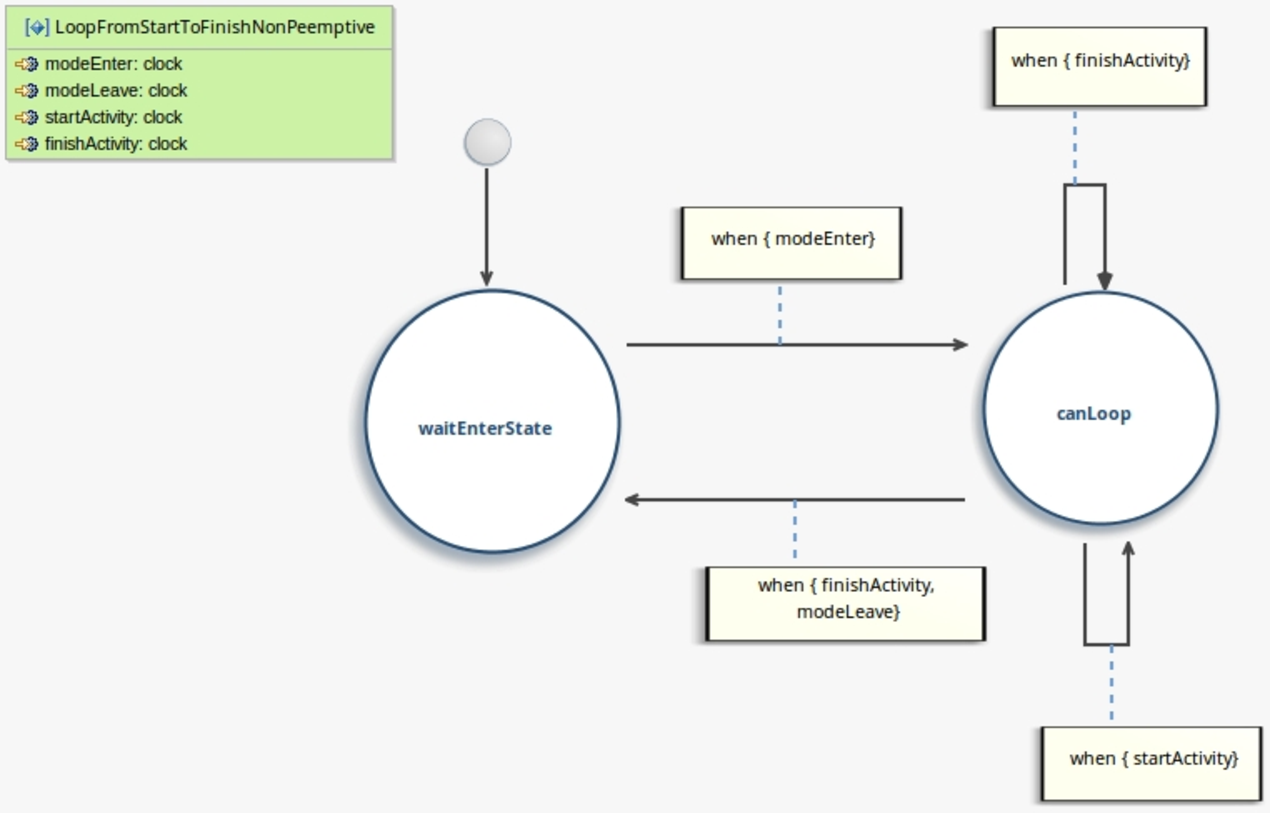
\includegraphics[width=.7\columnwidth]{examples/figs/LoopFromStartToFinishNonPreemptive}
	\caption{todo}
	\label{fig:looprelation}
\end{figure}



\begin{figure}
	\center
	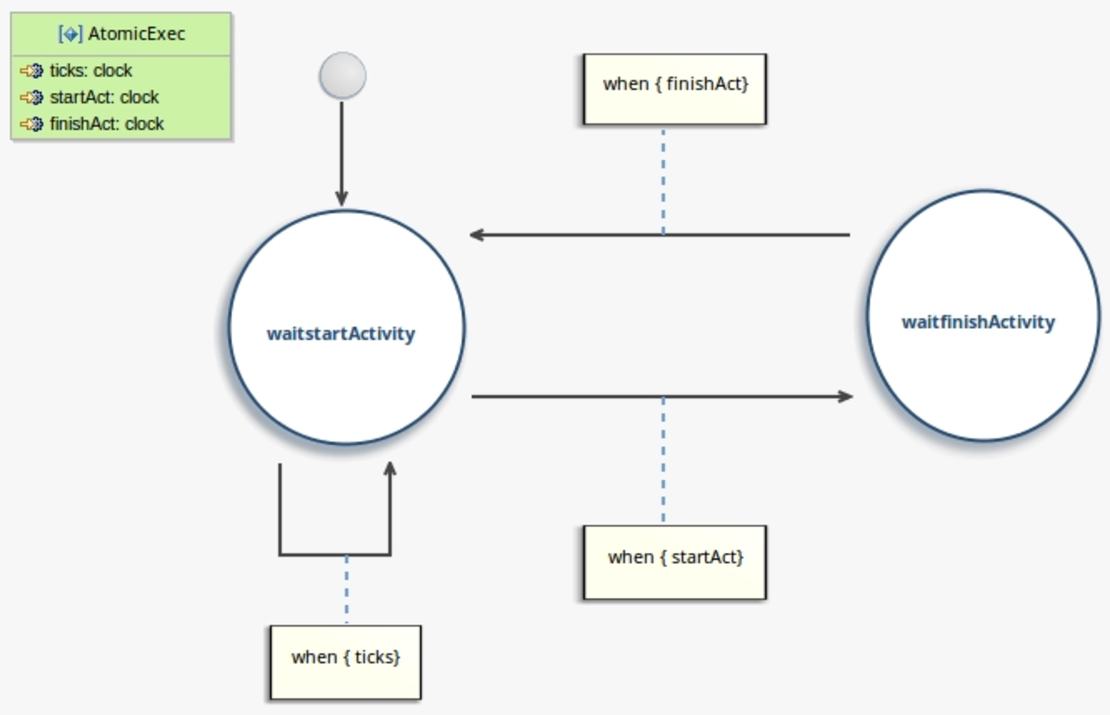
\includegraphics[width=.7\columnwidth]{examples/figs/AtomicExec}
	\caption{todo}
	\label{fig:atomicexec}
\end{figure}



Similar than the \emph{startActivityWhenEnter} operator, the \emph{AtomicActions} operator also defines a coordination between states and activities, but in this case, it deals with the temporal aspects of the coordination. The operator specifies how the time in the TFSM elapses during the execution of the activities that specify the on-entry action of a state. Thus, this coordination is also hierarchical, but in this case, only considers the timing aspects. In these languages, the time is represented differently. In the TFSM language, each state machine has a \emph{localClock} used to measure the time while the Activity language is untimed. The local clock is a \emph{FSMClock}, which defines a \dse named \emph{ticks} whose occurrences represent a physical time increment. In the Activity language, the duration of activities can be represented as the time between the \dse \emph{startActivity} and \dse \emph{finishActivity}. Thus, to coordinate the time, it is necessary to specify the number of \emph{ticks} of the local clock between the occurrence of the \dse \emph{startActivity} and \emph{finishActivity}. In this operator, we propose to enforce the execution of the ``internal'' activity to be atomic with respect to the time in the TFSM model. As a result, there is no occurrence of the \dse ticks of the corresponding local clock during the execution of the activity. 

In \bcool, we implement an operator named \emph{AtomicActions} (Listing~\ref{lst:bcoolStartActivityWhenEnter}: line 12) that specifies how time is consumed during the execution of the activities that are represented by states. It selects instances of \dse \emph{startActivity} and \emph{finishActivity} by using their context. As a result, the pairs selected identify the starting and finishing of an activity. To select the activities that represent a state, we use the onEnterAction. Then, we use the selected instances of \dse entering to select instances of \dse ticks of the corresponding local clock (Listing~\ref{lst:bcoolStartActivityWhenEnter}: line 13). To do so, we query the context of \dse \emph{entering} to get the localClock, and then, we compare with the context of the \dse ticks. To express the coordination rule, we rely on the event relation \emph{AtomicExec}. The event relation accepts three events as parameters: \emph{ticks}, \emph{startAct} and \emph{finishAct}. While the event ticks represents the ticking of the local clock, the startAct and finishAct events represent respectively the starting and finishing of an activity. Figure~\ref{fig:atomicexec} illustrates the state-based representation of the event relation that is made of two states named \emph{waitstartActivity} and \emph{waitfinishActivity}. In \emph{waitstartActivity} state, the event ticks is allowed to occur, thus making the time elapse. When the startAct event happens, the \emph{waitfinishActivity} state is reached and the event ticks is forbidden to occur, \ie the time in the TFSM does not elapse. Only when the event finishAct happens, the \emph{waitstartActivity} state is reached, and \emph{ticks} is allowed to occur again. In the operator, we use this relation to make the execution of the activities atomic, \ie there is no occurrence of the \dse ticks of the corresponding local clock during the execution of the activity.

In this section, we used \bcool to define a set of coordination operators that deal with both control and timing aspects of the coordination between states and activities. Unlike hierarchical coordination frameworks where the semantics is hidden, these operators explicitly specify how the hierarchical coordination is implemented. This specification contains also the operator \emph{SyncFSMEventsAndActions} (Listing~\ref{lst:bcoolrunningexample}), however, for the sake of simplicity it is not shown. In the following section, we use this specification to coordinate the models of a surveillance camera system.
	   %  The specification also contains the operator defined in the previous section that enables the coordination of Action and FSMEvents by relying in theirs names (It is now shown in Listing). 

\begin{lstlisting}[language=bcool,
caption={Hierarchical operator between TFSM and Activity languages},
label={lst:bcoolStartActivityWhenEnter}, 
basicstyle=\scriptsize\ttfamily, backgroundcolor=\color{LGrey}, numbers=left, xleftmargin=2pt]
Operator  StartActivityWhenEnter (activityStart : ad::startActivity , activityStop : ad::finishActivity, enterState : tfsm::entering, leaveState : tfsm::leaving)
when ((activityStart.name = activityStop.name ) and (enterState.name = leaveState.name) and (activityStart.name = enterState.onEnterAction.name));
do 
	LoopFromStartToFinishNonPeemptive (enterState, leaveState, activityStart, activityStop)
end operator;
\end{lstlisting}


\begin{lstlisting}[language=bcool,
caption={Timing Hierarchical operator between TFSM and Activity languages},
label={lst:bcoolAtomicExec}, 
basicstyle=\scriptsize\ttfamily, backgroundcolor=\color{LGrey}, numbers=left, xleftmargin=2pt, firstnumber=6]
Operator AtomicActions (activityStart : ad::startActivity , activityStop : ad::finishActivity, enterState : tfsm::entering, leaveState : tfsm::leaving, timeTicks : tfsm::ticks)
when ((activityStart.name = activityStop.name ) and (activityStart.name=enterState.OnEnterAction.name ) and (enterState.owningFSM.localClock = timeTicks));
do 
	AtomicExec (activityStart, activityStop, timeTicks)
end operator;
\end{lstlisting}




